\documentclass{standalone}
\usepackage{tikz}
\begin{document}
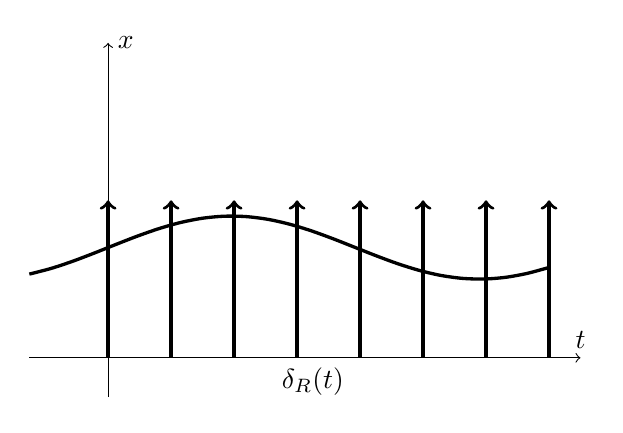
\begin{tikzpicture}[scale=2]
    \draw[->](0,-0.25)--(0,2)node[right]{$x$};
    \draw[->](-0.5,0)--(3,0)node[above]{$t$};

    \draw[very thick]plot[smooth, domain=-0.5:2.8](\x,{0.7+0.2*sin(2*\x r)});

    \draw[->,very thick](0,0)--(0,1);
    \draw[->,very thick](0.4,0)--(0.4,1);
    \draw[->,very thick](0.8,0)--(0.8,1);
    \draw[->,very thick](1.2,0)--(1.2,1);
    \draw[->,very thick](1.6,0)--(1.6,1);
    \draw[->,very thick](2,0)--(2,1);
    \draw[->,very thick](2.4,0)--(2.4,1);
    \draw[->,very thick](2.8,0)--(2.8,1);

    \node[below]at(1.3,0){$\delta_R(t)$};
\end{tikzpicture}
\end{document}